\documentclass{article}
\usepackage{tikz}

\title{ENGG102 Project 2A}
\author{Team E - Aminath Meesam Ali, Sienna Morris, Emily Durusovski}
\date{May 2025}

\begin{document}

\maketitle

\section{Forces on the cantilevered beam}

\begin{tikzpicture}[scale=0.1]
    % Draw the horizontal plane, dashed
    \draw[dashed] (0,0) -- (26.16, 0);
    % Draw the cantilevered beam, labeled with the length of L.
    \draw[thick] (0,0) -- (26.16,-26.16) node[midway, below] {$L$};    
    
    % Draw the force arrow (mg) 
    \draw[thick, -stealth, red] (26.16,-26.16) -- (26.16,-36.16);
    % Label the force
    \node[red] at (26.16,-31.16) [right] {$mg$};
    
    % Draw and the angle marker
    \draw (5,0) arc (0:-45:5);
    \node at (7,-2) {45°};
\end{tikzpicture}

\section{Forces on the incline}

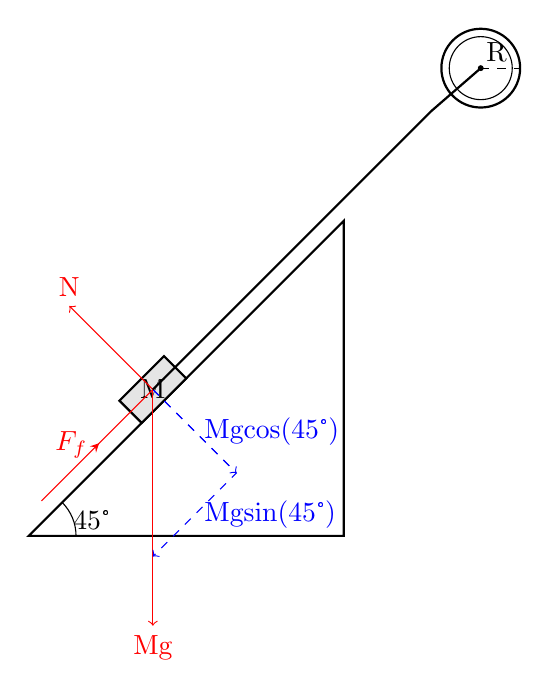
\begin{tikzpicture}

    % Draw pulley
    \draw[thick] (5.74,5.94) circle (0.5);
    \draw[fill=white] (5.74,5.94) circle (0.4); % Inner circle
    \draw[dashed] (5.74, 5.94) -- (5.74 + 0.5, 5.94);  
    \node at (5.74 + 0.2, 5.94 + 0.2) {R}; % Radius label
    \filldraw (5.74,5.94) circle (0.03); % Center dot

    % Draw the inclined plane
    \draw[thick] (0,0) -- (4,4) -- (4,0) -- cycle;
    
    % Label the angle (45 degrees)
    \draw (0.6,0) arc (0:45:0.6);
    \node at (0.8,0.2) {45°};

    % Drawing the M mass
    % Slope angle relative to the drawing
    \pgfmathsetmacro{\slopeangle}{atan2(4,-4)} 
    
    \begin{scope}[rotate around={\slopeangle:(2,2)}] % Rotate around midpoint
        \draw[thick, fill=gray!20] (2,2) rectangle ++(0.4,0.8); 
        \node at (2.2,2.4) {M}; 
        \coordinate (blockcenter) at (2.2,2.4);
    \end{scope}

    % Draw forces (both starting from center of mass M)
    \draw[->, red] (blockcenter) -- ++(135:1.5) node[above] {N}; % Normal force (perpendicular)
    \draw[->, red] (blockcenter) -- ++(270:3.0) node[below] {Mg}; % Weight force (downward)
    \draw[->, blue, dashed] (blockcenter) -- ++(135:-1.5) node[midway, right] {Mgcos(45°)}; % Vertical weight component
    \draw[->, blue, dashed] (blockcenter) -- ++(135:-1.5) -- ++(45:-1.5) node[midway, right] {Mgsin(45°)}; % Horizontal weight component
    \draw[red] (blockcenter) -- ++(45:-2.0) node[sloped, pos=0.5] {\tikz \draw[-stealth] (0,0) -- (2pt,0);} node[midway, left] {${F}_f$}; % Force due to friction

    % Draw connection to pulley
    \draw[thick] (blockcenter) -- ++(45:5.0) -- (5.74,5.94); 

\end{tikzpicture}

\end{document}
